\section{Methods}
\label{ch:DARPinMethods}

\subsection{Modified HDAC6 complex formation models}

We created two new HDAC6 complex formation models including DARPin-F10 as a competitor against Ub for HDAC6-Znf binding (Figure \ref{figure:darpinReactionModelSchemes}). These models are based on previously described "Symmetric" and "Asymmetric" model variants. Detailed model equations are described in Appendix \ref{appendix:DARPinModelsEquations}.

To compare original and modified HDAC6 complex formation models we uniformly sampled the rates and concentrations, as was previously described (Chapter \ref{ch:ReactionModels}) for original "Symmetric" and "Asymmetric" (Figure \ref{figure:darpinDensities}). We used two different predetermined concentrations of DARPin-F10. Based on \cite{guillard2017structural}, who report half maximal inhibitory concentration ($IC_{50}$) for DARPin-K27 and DARPin-K55 in the range between 2.4 to 67 nM in their experiments, we chose $34.7$ nM as an estimate for an active concentration of DARPin-F10, and  $34.7 \cdot 10^{-6}$ nM as a negligible DARPin concentration case. For on-rate of HDAC6 and DARPin-F10 binding $k_{HF}$ we chose $10^{6} \frac{1}{s\cdot M}$ - average rate of bimolecular reaction \cite{bionumbersbimolrate}. For dissociation constant $K_{HF}$ we used $90$ nM \cite{DarpinData}.

To determine the impact of DARPin-F10 concentration on uncoating we fixed all the other concentrations and rates, sampled widely in the range of $\pm$ 5 orders of magnitude around chosen literature value (as previously described in Methods \ref{ch:ReactionModelsMethods}). For these samples we simulated the modified reaction models for 2 hours of system time using the MATLAB ODE solver odeSD \cite{gonnet2012specialized}, such that the protein interactions lead to a steady-state distribution of the molecular species. We fitted both trajectories as a Hill equation using log-logistic function \texttt{LL.4()} from R package \texttt{drc}:

\begin{equation}
\epsilon=\frac{\epsilon_{max} - \epsilon_{min}}{1 + \big(\frac{EC_{50}}{[F]}\big)^n}
\end{equation}

where $\epsilon_{max}$ and $\epsilon_{min}$ are maximal and minimal drug efficacy, respectively, $[F]$ is DARPin F10 concentration, $EC_{50}$ is half maximal effective concentration of DARPin F10, and $n \ge 0$ is a Hill coefficient.

To compute the DARPin concentration $[F]_{effective}$ corresponding to experimentally observed uncoating (Figure \ref{figure:darpinUncoatingExperimental}) and viral growth (Figure \ref{figure:darpinGrowthExperimental}) reduction, we used the following formula:

\begin{equation}
[F]_{effective} = \exp\Big( \frac{1}{n}\cdot\log\big( \frac{\epsilon_{max}-\epsilon_{min}}{\epsilon_{max}\cdot\omega - \epsilon_{min}} - 1 \big) +\log(EC_{50}) \Big)
\label{eq:darpinEffectiveConcentration}
\end{equation}

where $\omega = \frac{1}{N_t}\sum_t \frac{x_{DARPin}(t)}{x_{WT}(t)}$ is an observed fraction of efficiency for observations $x$ at number $N_t$ of time points $t$.

Using the data \cite{DarpinData} provided by our collaborators we determined that for the uncoating experiment (Figure \ref{figure:darpinUncoatingExperimental}) at MOI = 30 PFU/ml corresponding efficiency of uncoating, compared to the wild type (WT) has been at approximately $\omega$ = 73\%. By comparing the averages of viral growth in presence of DARPin-F10 (Figure \ref{figure:darpinGrowthExperimental}) at MOI = 0.05 and 10 PFU/ml for data points >12 and $\ge$8 hours respectively, we determined that DARPin-F10 presence reduced viral growth respectively to $\omega$ = 31\% and $\omega$ = 11\% of WT. Using these values and Equation \ref{eq:darpinEffectiveConcentration} we can obtain estimates for the DARPin-F10 effective concentration (Table \ref{table:DARPinFittingCoefficients}).

\begin{table}[h!]
\centering
\caption[Fitted Hill equation parameters and effective DARPin-F10 concentrations]{Fitted Hill equation parameters and effective DARPin-F10 concentrations based on sampling HDAC6 complex formation models.}
\label{table:DARPinFittingCoefficients}

\begin{tabular}{p{5cm} p{3cm} p{3cm}}
\hline 
\textbf{Parameter} & \textbf{Asymmetric DARPin} & \textbf{Symmetric DARPin}\\
\hline
$n$ &                 1.37 $\pm$ 0.00 &    1.48$\pm$ 0.01\\
$\epsilon_{min}$ &    0.03 $\pm$ 0.00 &    -0.01$\pm$ 0.00\\
$\epsilon_{max}$ &    0.78 $\pm$ 0.00 &    0.65$\pm$ 0.00\\
$EC_{50}$, relative &          31.54 $\pm$ 0.05&    49.85$\pm$ 0.17\\
$EC_{50}$, $\mu$M &          1.1&    1.7\\
\hline
\multicolumn{3}{l}{$\omega$ = 73\%, uncoating assay}\\
$[F]_{effective}$, relative & 15.82 & 25.08\\
$[F]_{effective}$, $\mu$M & 0.5 & 0.9\\
\hline
\multicolumn{3}{l}{$\omega$ = 31\%, viral growth curves, MOI=0.05 PFU/ml}\\
$[F]_{effective}$, relative & 62.69 & 83.52\\
$[F]_{effective}$, $\mu$M & 2.2 & 2.9\\
\hline
\multicolumn{3}{l}{$\omega$ = 11\%, viral growth curves, MOI=10 PFU/ml}\\
$[F]_{effective}$, relative & 210.24 & 194.85\\
$[F]_{effective}$, $\mu$M & 7.3 & 6.8\\
\hline
\end{tabular}
\end{table}

\subsection{Functional analysis of literature available data}

We used the raw data for influenza infection for three different MOI = $10^{-4}$, $3$, $73$ reported in the supplement of \cite{rudiger2019multiscale}, to plot influenza infection total virus growth trajectory and fit it using asymptotic regression function \texttt{AR.3()} from R package \texttt{drc}:

\begin{equation}
f(x) = c + (d-c)\big(1-\exp(-\frac{t}{e})\big)
\label{eq:ar3function}
\end{equation}

The parameter $c$ is the lower limit at $t=0$, the parameter $d$ is the upper limit, and the parameter $e>0$ is determining the steepness of the increase with $t$.

Analogously, we fitted the WT DARPin viral growth curves provided to us by our collaborators \cite{DarpinData} (Figure \ref{figure:totalVirusFits}).

\begin{figure}
\begin{center}
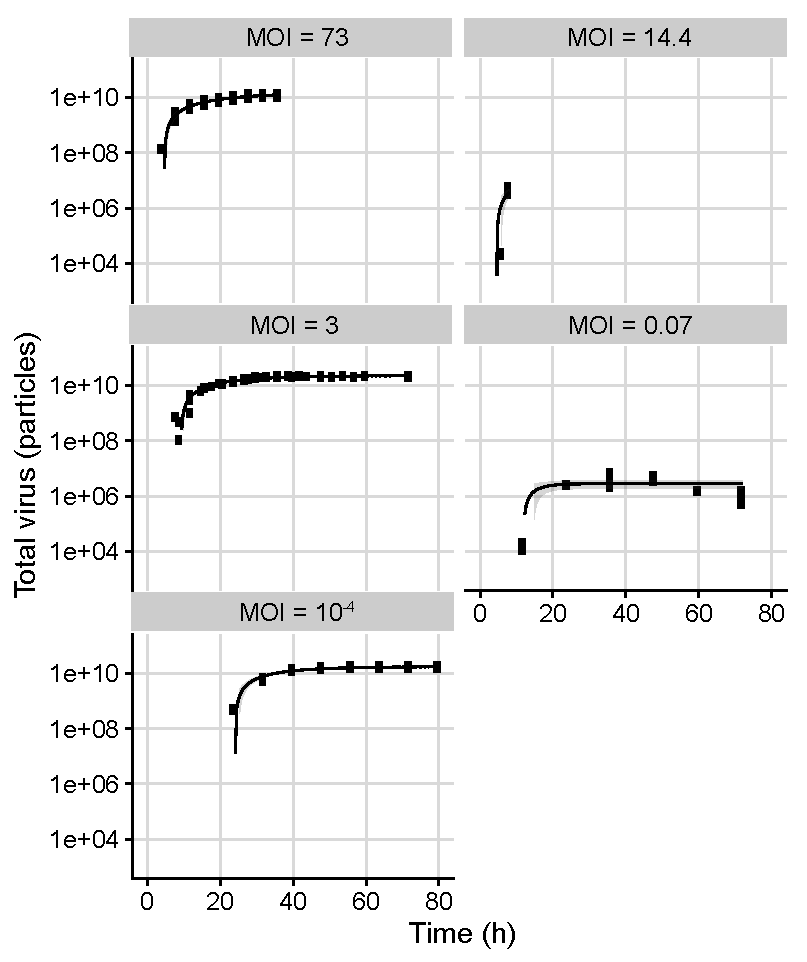
\includegraphics[width=0.8\textwidth, trim={0cm 0cm 0cm 0cm}, clip]{D_chapters/3_DARPinModels/fittingTotalVirus.pdf}
\caption[Total virus asymptotic regression fits]{Total virus asymptotic regression fits using \cite{rudiger2019multiscale, DarpinData} data.}
\label{figure:totalVirusFits}
\end{center}
\end{figure}

Our collaborators measure MOI in PFU/ml, while \cite{rudiger2019multiscale} used 50\% tissue culture infectious dose (TCID$_{50}$) assay to measure it. To convert PFU/ml units into approximate TCID$_{50}$ we used the Poisson distribution:

\begin{equation}
P = \exp(-MOI_{mean})
\end{equation}

where $MOI_{mean}$ is a mean number of infectious units per volume is expressed in PFU/ml units. For any titer expressed in TCID$_{50}$ P = 0.5, giving us $MOI_{mean} = -\log(0.5)$. Under the assumption that the protocol changes do not affect viral production, we convert PFU/ml to TCID$_{50}$ by dividing corresponding MOI measurements by $MOI_{mean}$. This gives us MOI = 10 PFU/ml = 14.4, and MOI = 0.05 PFU/ml = 0.07.

To calculate the delay time for each value of MOI we used Equation \ref{eq:ar3function} and compute the $\tau_{delay}$ value corresponding to $f(x) = 0$:

\begin{equation}
\tau_{delay} = -e\log(1+\frac{c}{d-c})
\end{equation}

We then fitted $\tau_{delay}$ as a function of MOI (Equation \ref{eq:delayMOI}) using R function \texttt{lm} from package \texttt{stats}.

To validate this equation, we digitized viral production curves reported in \cite{baccam2006kinetics, handel2007neuraminidase, handel2010towards, smith2011effect, miao2010quantifying, mohler2005mathematical} using the WebPlotDigitizer \cite{Rohatgi2020} tool, fitted and computed corresponding $\tau_{delay}$ values. For MOI we either used the reported values, or calculated them based on the number of cells and virus used in the experiments (Table \ref{table:delayTauValidation}, Figure \ref{eq:delayMOI}).

\begin{table}[h!]
\centering
\caption[$\tau_{delay} = f(MOI)$ validation]{$\tau_{delay} = f(MOI)$ validation based on digitized literature data.}
\label{table:delayTauValidation}

\begin{tabular}{p{2cm} p{2cm} p{2cm} p{2cm} p{4cm}}
\hline 
\textbf{Data} & \textbf{MOI} & \textbf{$\tau_{delay}$ (h)} &  \textbf{Species} & \textbf{Strain}\\
\hline
\cite{baccam2006kinetics} & $4\cdot 10^{-5}$ & 27.4 & human & A/Hong Kong/123/77 (H1N1)\\
\cite{handel2007neuraminidase} & $1\cdot 10^{-4}$ & 24.1 & human & A/Texas/91 (H1N1)\\
\hline
\cite{handel2010towards} & $1.7$ & 32.0 & mouse & A/Puerto Rico/8/34 (H1N1)\\
\cite{smith2011effect} & $1\cdot 10^{-5}$ & 13.5 & mouse & A/Puerto Rico/8/34 (H1N1) with PB1-F2(1918)\\
\cite{smith2011effect} & $1\cdot 10^{-5}$ & 19.2 & mouse & A/Puerto Rico/8/34 (H1N1)\\
\cite{miao2010quantifying} & $5\cdot 10^{-3}$ & 7.6 & mouse & A/Hong  Kong/X31 (H3N2)\\
\hline
\cite{schulze2009infection} & 0.025 & 15.0 & MDCK & A/Puerto Rico/8/34 (H1N1) NIBSC\\
\cite{schulze2009infection} & 0.025 & 17.5 & MDCK & A/Puerto Rico/8/34 (H1N1) RKI\\
\cite{schulze2009infection} & 0.002 & 16.5 & MDCK & WSN/67/2005 (H3N2)\\
\cite{mohler2005mathematical} & 0.025 & 14.2 & MDCK & A/equine/ Newmarket /1/93 (H3N8)\\
\hline
\end{tabular}
\end{table}

To analyze the infectious fraction change over time we plotted the data reported in \cite{rudiger2019multiscale, schulze2009infection}, and fitted it as a parallel slope model using R function \texttt{lm} from package \texttt{stats}:

\begin{equation}
\log(\text{Infectious fraction}) = a + b \cdot t
\end{equation}

where $t$ is time, $b$ is a slope coefficient, and $a$ is an intercept, conditional on MOI \cite{rudiger2019multiscale} or viral strain \cite{schulze2009infection} (Table \ref{table:linearFitsInfectiousFraction}).

\begin{table}[h!]
\centering
\caption[Linear fits of infectious fraction]{Linear fits of infectious fraction}
\label{table:linearFitsInfectiousFraction}

\begin{tabular}{p{2cm} p{2cm} p{2cm} p{2cm} p{4cm}}
\hline 
\textbf{Data} & $b$ & $a$ &  \textbf{MOI} & \textbf{Strain}\\
\hline
\cite{rudiger2019multiscale} & -0.13 & 1.73 & $10^{-4}$ & PR/8/34 (H1N1) RKI\\
\cite{rudiger2019multiscale} & -0.13 & 0.22 & 3 & PR/8/34 (H1N1) NIBSC\\
\cite{rudiger2019multiscale} & -0.13 & -2.70 & 73 & PR/8/34 (H1N1) NIBSC\\
\hline
\cite{schulze2009infection} & -0.18 & -8.97 & 0.025 & PR/8/34 (H1N1) NIBSC\\
\cite{schulze2009infection} & -0.18 & -4.52 & 0.025 & PR/8/34 (H1N1) RKI\\
\cite{schulze2009infection} & -0.18 & -5.90 & 0.002 & WSN/67/2005 (H3N2)\\
\hline
\end{tabular}
\end{table}

\subsection{Influenza infection model selection}

We used two chronic and seven depletion influenza infection models, which are described in detail in Appendix \ref{appendix:compartmentalModelEquations}. We simulated these models for 80 hours of  system time using MATLAB solvers \texttt{ode23} (with extra condition that all the variables stay positive during the simulation) or \texttt{dde23} (for delay models).

We assume that at the start of the simulation all the cells are target cells $T_0 = 6.7 \cdot 10^6$ \cite{saenz2010dynamics}, $E_0$, $I_0$, $R_0$ = 0. The number of viral particles is $V_0 = T_0 \cdot MOI$, with number of infectious viral particles being determined based on initial total virus and infectious fraction $V_i0 = V_0 \cdot i_{fraction}$ (for detailed notation see Appendix \ref{appendix:compartmentalModelEquations}).

For each of the models we first manually selected a set of parameters which seemed to provide a decent fit to literature data \cite{rudiger2019multiscale}. Using this pre-selected set as a starting point, we generated 49 latin hypercube samples $\pm$ 1 order of magnitude around that manually selected parameter set, with the exception of $i_{Fraction}$, EC$_{50}^{Target}$ and n$^{Target}$, which were sampled in [0,1], [0, $T_0$], and general vicinity of pre-selected value respectively. To determine the best fit, we ran MATLAB function \texttt{fmincon} for each of those samples, including the pre-selected set. We used objective function

\begin{equation}
F = \sum_t \sum_i M_i \cdot \frac{\log (\big| x^i_{simulated} - x^i_{experimental} \big|)^2}{\log (\sigma^i_{experimental})^2}
\end{equation}

where $t$ is time at which experimental measurement happened, $i$ index of measured variable, $x^i_{simulated}$ is a value of the variable $i$ predicted by the model, $x^i_{experimental}$ is an experimentally measured value of the variable $i$, $\sigma^i_{experimental}$ is an experimentally reported standard deviation of the variable $i$, and $M_i$ is a multiplication matrix which checks whether the predicted value is over 0. Delay solvers in MATLAB do not have an option for non-negative solutions, so we penalize our model if the simulated value is negative:

\begin{equation}
M_i =
\begin{cases}
1 & \mbox{if } x^i_{simulated} \ge 0\\
10000 & \mbox{if } x^i_{simulated} < 0
\end{cases}
\end{equation}

Resulting lowest objective function values for each of the influenza infection models are reported in Table \ref{table:ModelObjFunction}. To validate our models, we compared them against literature data \cite{schulze2009infection}. We used the fitted parameter sets corresponding to these lowest objective function values, and simulated them with new initial conditions $T_0$ equal to the starting target cell numbers in \cite{schulze2009infection}, and corresponding values of MOI. Resulting plots are shown in Appendix \ref{appendix:compartmentalModelFitValidation}.

\subsection{Simulating drug-like effect of DARPin-F10}

We modified models T$_{Hill}$IRVV$_i$, delay $\tau = const$ and T$_{Hill}$IRVV$_i$, delay $\tau = f(\text{MOI})$ to include a DARPin-F10 drug-like effect. We created amantadine-like DARPin-F10 models which modify infection rate $\beta$, and neuraminidase inhibitor-like DARPin-F10 models which modify viral production rate $p$ as detailed in Appendix \ref{appendix:compartmentalModelEquations}.

We simulated these modified models for MOI = 0.05 PFU/ml = 0.07 first as is, and then with DARPin-F10 concentrations and parameters as determined by dose-response fits of modified HDAC6 complex formation models "Asymmetric DARPin" and "Symmetric DARPin" (Table \ref{table:DARPinFittingCoefficients}).

We then compared the results of the simulation (Figures \ref{figure:amantadineLikeF15}, \ref{figure:amantadineLikeF210}, \ref{figure:amantadineLikeF62}, \ref{figure:neuraminidaseInhibitorLikeF15}, \ref{figure:neuraminidaseInhibitorLikeF210}, \ref{figure:neuraminidaseInhibitorLikeF62}) with experimentally predicted viral growth curves \cite{DarpinData}. For ease of comparison, we normalized the experimental values to simulated virus production value at 48h for no DARPin case.

